\documentclass[10pt, letterpaper]{article}
        \usepackage[utf8]{inputenc}
        \usepackage[margin=1in]{geometry}
        \usepackage{fancyhdr}
        \usepackage{titling}
        \usepackage{enumitem}
        \usepackage{mathtools}
        \usepackage{amssymb}
        \usepackage{xfrac}
        \usepackage{booktabs}
        \usepackage{graphicx}
        \usepackage{wrapfig, blindtext}
        \usepackage{hyperref}
        \usepackage{enumerate}
        \usepackage{multicol}
        

        
        \setlength{\parindent}{0pt}

\title{Journal 2}
        \author{Sudhan Chitgopkar}
        \date{\today}
        
        % headers -- no need to change
        \pagestyle{fancy}
        \fancyhf{}
        \lhead{2016 Election JCC}
        \chead{UGAMUNC XXVII}
        \rhead{\thedate}

\begin{document}

Dear Delegates, \\

It is our pleasure to welcome you all to the twenty-seventh annual UGA
Model United Nations Conference, UGAMUNC XXVII. We hope that your
experience at this conference will teach you a little bit more about the
events surrounding this committee, different tactics of negotiation, or
even just a little more about yourselves! In the 2016 Election
Interference Crisis Committee at UGAMUNC, you'll be experiencing things
a bit differently than your fellow high school delegates. \\

Before we explain further, we would like to introduce ourselves, as well
as our chairs and co-chairs. The crisis director for the Federal Bureau
of Investigation (US) is Meredith Van De Velde
(\texttt{\href{mailto:meredithvandevelde@uga.edu}{meredithvandevelde@uga.edu}}).
Meredith is a fourth-year Computer Science and International Affairs
major at UGA. Meredith has been involved in Model UN for eight years,
both in high school and college, and currently serves as the Secretary
General of the UGA Model United Nations team. \\

The crisis director for the Internet Research Agency (Russia) side is
Miranda Bourdeau \newline
(\texttt{\href{mailto:bourdeau.miranda@gmail.com}{bourdeau.miranda@gmail.com}}).
Miranda is a fourth-year International Affairs, Political Science, and
Economics major at UGA. This is Miranda's fourth year of doing Model UN
and her third year on the UGA team. She currently serves as Collegiate
Conference Director for the UGA MUN team. \\

The chair of the United States committee will be Matthew Li
(\href{mailto:Matthew.Li@uga.edu}{\underline{Matthew.Li@uga.edu}}).
Matthew is a first-year Biochemistry \& Molecular Biology major with a
Spanish minor and maybe a masters in Comparative Biomedical Sciences
(who knows!). This is his fifth year doing Model UN, and he looks
forward to seeing all of you work in committee. The co-chair of the
United States committee will be Alice Ware
(\href{mailto:alice.ware@uga.edu}{\underline{alice.ware@uga.edu}}).
Alice is a first-year Statistics and Theatre major at UGA. This is her
first year on the UGA MUN team and is excited to experience UGAMUNC on
the other side of the dias. \\

The chair of the Russia committee will be Nic Rasool
(\href{mailto:chaudhry.rasool@uga.edu}{\underline{chaudhry.rasool@uga.edu}}).
Nic is a second-year Biological Engineering and Philosophy double major
with minors in Biology and German. This is his sixth year doing Model UN
and second year on the UGA MUN team, and is looking forward to seeing
crisis arcs come to fruition. The co-chair of the Russia committee will
be Logan King
(\href{mailto:logan.king@uga.edu}{\underline{logan.king@uga.edu}};
they/them). Logan is a second-year History and Political Science major
at UGA with minors in Geography and Korean. This is their third year
doing Model UN and their first year on the UGA MUN team; they are
looking forward to fruitful committee sessions! \\

We know that you'll all do a fantastic job bringing your role to life in
conference. If you have any questions please don't hesitate to contact
us. From now until UGAMUNC, start delving deeper into your character and
building your crisis arc. We can't wait to see you all in action. \\

Once again, welcome to UGAMUNC XXVII! \\

Miranda Bourdeau and Meredith Van De Velde\\
Co-Crisis Directors, 2016 Election Interference JCC

\newpage
\tableofcontents
\newpage

\section{Rules and Procedure}

\subsection{General Rules}

While other delegates at UGAMUNC may be placed in traditional General
Assembly-style Model United Nations committees, the 2016 Election
Interference committee at UGAMUNC will run as a crisis committee. While
you should still familiarize yourself with the UGAMUNC Rules and
Procedure document to brush up on parliamentary procedure, this
committee will vary from the typical format. Please familiarize yourself
with the following rules specific to this committee, and once again, if
you have any questions, feel free to reach out to us at
\texttt{\href{mailto:meredithvandevelde@uga.edu}{meredithvandevelde@uga.edu}}
or
\texttt{\href{mailto:bourdeau.miranda@gmail.com}{bourdeau.miranda@gmail.com}}. \\

\begin{itemize}
\item
  \textbf{This committee is loosely based on election interference in
  the 2016 US presidential election.} This is the general topic of our
  crisis committee, and as members of the FBI or IRA, this will be the
  focus of much of the conversation for the weekend. However, you are
  more than welcome to focus on related issues of the times or alter the
  path of history forever.

\item
  \textbf{While this is a historical committee, you have the freedom to
  alter history.} This committee is to be set starting on {[}date{]},
  only a few months before election results are called. While members of
  this body should consider any events that took place prior to
  {[}date{]} as historical facts in this committee, any events that
  occurred after that date will not automatically occur even if they are
  mentioned in the background guide to provide context. Characters in
  this body have a chance to rewrite fate in the manner they choose,
  including changing the results of the election or escalating the
  situation further.

\item
  \textbf{Utilize crisis notes to accomplish your goals in committee and
  craft your crisis arc.} While the main method of negotiation in a
  typical General Assembly-style committee stems from typical speaking
  time work in committee, in a crisis committee, much of the work you do
  will be on your own through crisis notes. These are letters that your
  character will write to crisis, a body outside of the committee room,
  to accomplish something without the committee's knowledge. A good
  crisis note not only explains, in detail, what to do, but it also
  explains very specifically how to do it. These notes will be addressed
  to a fictional person that has some relation to your character.
  ``Crisis'' (UGAMUNC staff and your crisis director) will answer these
  notes as if they were this fictional person, responding as that person
  would under the circumstances from the context you set out. Only
  address a note to crisis if you have a question about the way
  committee is going. There are many fantastic resources that better
  explain crisis notes in detail, but a starting point can be found
  \texttt{\href{http://bestdelegate.com/the-three-crisis-notes-to-send-at-the-beginning-of-any-model-un-crisis-committee/}{here}})

\item
  \textbf{Because this is a crisis-style committee, write directives,
  not resolutions.} Although they are very similar, directives are the
  typical formal paper written in a crisis committee, not resolutions.
  Directives are less formal, are normally titled, and are generally
  more straightforward. They are intended to utilize the powers present
  in the committee to quickly address the crisis at hand or any related
  issues.


\item
  \textbf{Represent your understanding of your character.} This is a
  modern crisis committee, meaning that much of the context surrounding
  this committee has been heavily researched and reported upon. Use this
  to your advantage; do some research! Each character is unique, and
  therefore has unique goals and relationships among members of the
  committee. That said, be sure to represent your character's beliefs
  and not simply your own. While you may not be prepared for the updates
  which crisis will present to you, you can at least understand the
  character you have been assigned and react to crisis in the way they
  would.


\item
  \textbf{This committee is English only.} Even if you can speak
  Russian, there will be no advantage given to any delegate who chooses
  to write crisis notes or give speeches in Russian. While we certainly
  respect cultural accuracy, we don't want to exclude other delegates in
  committee who may not speak Russian (including your chairs, co-chairs,
  and crisis directors).
 
\item
 
  \textbf{Position papers will be due February 1, 2021.}
  Your position paper should explain what approach your character will
  take regarding personal actions, how you plan to interact with other
  delegates, and how you will respond to the main issues in the
  committee. Qualifying position papers for this committee will be one
  page and 1.5 spaced, 12 point Times New Roman font, one-inch margins,
  as well as a standard and consistent citation format of your choosing
  (i.e. MLA, Chicago, etc.). Please submit these position papers
  directly to either Meredith
  (\texttt{\href{mailto:meredithvandevelde@uga.edu}{meredithvandevelde@uga.edu}})
  or Miranda
  (\texttt{\href{mailto:bourdeau.miranda@gmail.com}{bourdeau.miranda@gmail.com}})
  depending on your committee. We have attached some resources below to
  help you get started. Happy writing! \\
\end{itemize}

\subsection{Position Paper Resources}
\begin{itemize}
\item
Best Delegate:
\texttt{\href{https://bestdelegate.com/how-to-write-a-winning-position-paper/}{https://bestdelegate.com/how-to-write-a-winning-position-paper/}} 
\item
NMUN:
\texttt{\href{https://www.nmun.org/assets/documents/NMUNPPGuide.pdf}{https://www.nmun.org/assets/documents/NMUNPPGuide.pdf}} 
\item
AMUN example papers:
\texttt{\href{https://www.amun.org/sample-paper-1/}{https://www.amun.org/sample-paper-1/}} 
\end{itemize}

\newpage

\section{Expectations of a Joint Crisis Committee (JCC)}

While joint crisis committees, more commonly referred to as JCCs, are
common on the collegiate conference circuit, they are rare among high
school conferences. This year, UGA Model UN is seeking to change that
with this 2016 election interference committee, the first joint crisis
committee that UGAMUNC has ever run. \\

As the name implies, JCCs are crisis committees, meaning that they
follow typical crisis procedure. Therefore, an understanding of crisis
committee procedure and crisis arcs will be helpful. For more
information on the parliamentary procedure expected in a crisis
committee at UGAMUNC, please refer to the delegate handbook found at
\texttt{\href{https://www.ugamunc.com}{https://www.ugamunc.com}}. \\

Like typical crisis committees, each committee within a JCC has its own
Chair, Co-Chair, Crisis Director, and Crisis Staffers. JCCs function in
more than one physical committee room. In our case, the JCC will be
operating across two rooms - the Federal Bureau of Investigation (FBI)
and the Internet Research Agency (IRA). However, every committee in a
JCC is interconnected, both thematically and practically. Joined by a
central issue, the committees in a JCC interact with one another:
delegates in each JCC committee can interact with the delegates in other
committees. \\

Both sides of this committee will be heavily involved in the issue of
2016 election interference, but they will be operating on opposite sides
of the issue. JCCs are themed around wars (cold or regular) and have a
high likelihood of war games happening. The ``back room,'' commonly
known as ``crisis,'' will be the same room and group of writers for both
committees. This allows the actions in one committee to quickly affect
the other. It also allows for communication across rooms, either
directly from one delegate to another, or indirectly through crisis. \\

The format of this committee may lead you to believe that the most
important aspect is your ``behind-the-scenes'' work as a character
through crisis. However, the best delegates in a crisis committee find
the balance between writing directives and crisis notes that further
your character's short and long-term goals in committee. \\

\section{Disclaimer on the topic of this Committee}

This committee is not only unique due to its format as a JCC, but also
because of its modern setting. The events to be discussed in this
committee happened only a couple of years ago, and as such, we
understand that delegates may have personal opinions on the context
surrounding the committee. We ask that all delegates put aside their own
personal political ideology for the duration of this committee to fully
participate as your assigned characters. \\

Additionally, we would like to underscore that any events that are
discussed in this background guide are real. Any instances of election
interference have been found as fact from reputable sources, all of
which are referenced in this document.\footnote{Mueller, Robert S., et
  al. \emph{Report on the Investigation into Russian Interference in the
  2016 Presidential Election: Submitted Pursuant to 28 C.F.R.
  §600.8(c)}. U.S. Department of Justice, 2019.} \\

As always, please be respectful of other delegates, the Chair and
Co-Chair of the committee, and the Crisis Staffers.

\newpage
\section{Background of Committee - both sides}

\subsection{Summary of Russian Interference}

In July 2016, the FBI opened an investigation into the Russian
government's attempt to influence the 2016 presidential election,
including any possible connections between the Trump campaign and
Russian operatives. The campaign from the Russians was dual-pronged:
Russia directly attacked members of the Democratic National Committee
(DNC) as well as passively spreading information on social media. \\

As early as December 2015, The Internet Research Agency (IRA), a Russian
online propaganda operation, conducted a social media campaign ``to
advocate for President-elect Trump as early as December 2015,''
according to a US intelligence community report.\footnote{\emph{Assessing
  Russian Activities and Intentions in Recent US Elections}. Office of
  the Director of National Intelligence, National Intelligence Council,
  2017.} In April 2016, the IRA began to officially produce, purchase,
and post advertisements on U.S. social media and other online sites
expressly advocating for the election of then-candidate Trump or
expressly opposing Clinton. By June, the IRA, began to organize
political rallies, including pro-Trump or anti-Clinton rallies
throughout the United States, including in Florida, Pennsylvania, and
New York.\footnote{Kiely, Eugene. ``Timeline of Russia Investigation.''
  \emph{FactCheck.org}, 27 Apr. 2020,
  www.factcheck.org/2017/06/timeline-russia-investigation/.}
Additionally, throughout Fall 2016, IRA-managed social media accounts,
including Instagram account ``Blacktivist,'' posted messages as part of
a larger campaign to suppress the minority vote in the 2016 US
presidential election. This included encouraging minority groups to vote
for third party candidates such as Green Party candidate Jill
Stein.\footnote{Windrem, Robert. ``Russians Launched pro-Jill Stein
  Social Media Blitz to Help Trump Win Election, Reports Say.''
  \emph{NBCNews.com}, NBCUniversal News Group, 22 Dec. 2018,
  www.nbcnews.com/politics/national-security/russians-launched-pro-jill-stein-social-media-blitz-help-trump-n951166.} \\

Simultaneously, President Putin sanctioned an influence campaign during
2016 aimed at the US presidential election. Russian intelligence
services gained access to the computer network of Democratic Party
officials and released the hacked material to WikiLeaks and others ``to
help President-elect Trump's election chances,'' according to the
aforementioned IC report. \\

\subsection{Digital Election Interference as a Strategy}

Although Russian interference in the 2016 US presidential election is by
far the most public instance of election interference, it is not the
first. Election interference can be conducted through dissemination of
disinformation, as was done for Russia in 2016, but it can also involve
directly compromising election infrastructure, such as directly hacking
election machines or setting up fake absentee ballot dropboxes. Two
examples of elections prior to the 2016 US presidential election that
experienced interference through social media disinformation campaigns
are the 2012 Mexican presidential election and Russian interference in
Ukrainian elections from 2004 through the present. \\

The 2012 Mexican presidential election was heavily influenced by mass
Twitter campaigns by the Institutional Revolutionary Party, or PRI, to
trend hashtags in favor of their candidate's campaigns.\footnote{Vega,
  Ana Francisca. ``Spambots Driving Mexican Twitter Users Crazy Ahead of
  Presidential Election.'' \emph{Slate Magazine}, Slate, 22 June 2012,
  slate.com/technology/2012/06/spambots-on-twitter-for-mexican-presidential-candidates-like-the-pri-s-enrique-pena-nieto.html.}
The PRI used tens of thousands of bots, or user accounts programmed to
tweet automatically.\footnote{Orcutt, Mike. ``Twitter Mischief Plagues
  Mexico's Election.'' \emph{MIT Technology Review}, MIT Technology
  Review, 2 Apr. 2020,
  www.technologyreview.com/2012/06/21/185262/twitter-mischief-plagues-mexicos-election/.}
In some cases, they even paid real people to simultaneously tweet the
same message.\footnote{``Twittergate: Is Mexico's PRI Paying for
  Tweets?'' \emph{UnivisionNews1}, 2012,
  www.youtube.com/watch?v=XGRXxct3L4A.} Although the PRI used the most
effective strategy in the 2012 election, allowing their candidate,
Enrique Peña Nieto to win 38\% of the vote, all three dominant political
parties in Mexico have used bots in various elections at the national
and state level.\footnote{Orcutt, Mike. ``Twitter Mischief Plagues
  Mexico's Election.'' \emph{MIT Technology Review}, MIT Technology
  Review, 2 Apr. 2020,
  www.technologyreview.com/2012/06/21/185262/twitter-mischief-plagues-mexicos-election/.} \\

Russia utilized sophisticated cyber techniques in an election in Ukraine
as early as 2014. In the 2014 election, however, Russian hackers
infiltrated Ukraine's central election commission to spread a virus that
would have changed the results of the election in favor of a fringe
ultra-nationalist party, Right Sector, had Ukrainian cybersecurity
experts not detected the malware less than an hour before the election
results were announced.\footnote{SHULMAN, STEPHEN, and STEPHEN BLOOM.
  ``The Legitimacy of Foreign Intervention in Elections: the Ukrainian
  Response.'' \emph{Review of International Studies}, vol. 38, no. 2,
  2012, pp. 445--471., www.jstor.org/stable/41485557. Accessed 29 Oct.
  2020.} In addition to their direct cyberattack, Russian state media
still reported the fake results, showing the ultra-nationalists winning,
and attempted to spread that information on social media.\footnote{``THE
  FUTURE OF POLITICAL WARFARE: RUSSIA, THE WEST, AND THE COMING AGE OF
  GLOBAL DIGITAL COMPETITION.'' \emph{Brookings Institution}, Mar. 2018,
  www.brookings.edu/wp-content/uploads/2018/03/fp\_20180316\_future\_political\_warfare.pdf.}
Many experts consider these Russian disinformation campaigns as
precursors to the country's actions in American elections in 2016 and
recommend decisive action to stop any similar actions in
2020.\footnote{Tennis, Maggie. ``Russia Ramps up Global Elections
  Interference: Lessons for the United States.'' \emph{Russia Ramps up
  Global Elections Interference: Lessons for the United States
  \textbar{} Center for Strategic and International Studies}, 20 Oct.
  2020,
  www.csis.org/blogs/technology-policy-blog/russia-ramps-global-elections-interference-lessons-united-states.} \\

\subsection{International Law in Election Interference}

\begin{wrapfigure}{r}{0pt}
\centering
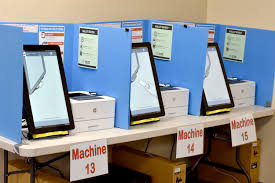
\includegraphics[scale = 0.7]{image4.jpg}
\end{wrapfigure}

There are several methods of digital election interference. Perhaps most
obvious is actual interference in the election process. In some
countries, electronic voting and vote tabulation systems are over a
decade old, maybe even no longer manufactured.\footnote{Norden,
  Lawrence, et al. ``Election Security.'' \emph{Brennan Center for
  Justice}, 29 June 2017,
  www.brennancenter.org/issues/defend-our-elections/election-security.}
This means it is nearly impossible to conduct maintenance tests on the
machines, which introduces the possibility of inaccuracy when tabulating
votes. In addition, these systems are not updated with the latest
digital security protections, so they are more susceptible to
interference in the election process. They can very easily be hacked and
see votes not counted or even changed to sway the results of an
election. As hacking capabilities have advanced, older voting machines
become more vulnerable to attack. \\

Less obvious but more prevalent lately is running disinformation
campaigns through social media platforms. Some foreign state-run media
sources infuse the political agenda of their home country when reporting
in the United States. In fact, Moscow's multimedia ``propaganda
machine'' has heavily pushed the virtues of Trump and sowed
disinformation on the corruption of American democracy.\footnote{Friedman,
  Uri. ``Russia's Election Meddling Is Part of a Bigger Story.''
  \emph{The Atlantic}, Atlantic Media Company, 24 July 2017,
  www.theatlantic.com/international/archive/2017/07/legal-ways-interfere-election/534057/.}
Social media has also been a source of disinformation campaigns for digital election interference. Facebook and Twitter especially have recently faced increased scrutiny for their protocols running political ads and removing false information regarding politics. It is relatively simple for foreign operatives to either purchase ad spaces or create thousands of fake accounts that promote the spread of disinformation supporting a certain political agenda.\footnote{Parks, Miles. ``5 Ways Election Interference Could (And
  Probably Will) Worsen In 2018 And Beyond.'' \emph{NPR}, NPR, 27 Jan.
  2018,
  www.npr.org/2018/01/27/579683042/5-ways-election-interference-could-and-probably-will-worsen-in-2018-and-beyond.} \\

With so many people on social media in this day and age, disinformation
campaigns can be extremely successful by reaching a large audience in a
short amount of time. Considering foreign agents are able to amplify
already-existing divisions in American politics through disinformation
campaigns, it is up to this committee to decide how to best handle
foreign infiltration of our election process in order to uphold the
values of democracy. \\

The question is, however, is either method of digital election
interference considered illegal in terms of international law? Its
answer is not straightforward. International law prohibits countries
from ``coercively interfering in each other's domestic affairs, whether
social, political, or economical.''\footnote{``TU Law Professor Explores
  the Role of U.S. and International Law to Mitigate Foreign
  Interference in Elections -.'' \emph{College of Law}, 29 Apr. 2020,
  law.utulsa.edu/cybersecurity-election-interference-kilovaty/.}
However, digital election interference may not be considered coercive.
After all, no one is being forced to do anything or threatened to vote
in a certain way. In this manner, hacking voting machines or spreading
disinformation on social media, although considered interfering in a
country's domestic affairs, would not be considered violating
international law. \\

It is also possible to consider hacking voting machines an act of
espionage. Spying has traditionally been understood as a violation of
domestic, but not international, law.\footnote{Ohlin, Jens David.
  Cornell Law Faculty Publications, 2017, pp. 1580--1582, \emph{Did
  Russian Cyber Interference in the 2016 Election Violate International
  Law?}} However, some people consider election interference to be a
violation of national sovereignty.\footnote{\emph{Ibid.}} Proponents of
this perspective argue that a country loses its right to govern itself
without forcible interference from outside bodies when its elections are
tampered with. It is believed that by not being able to accurately
choose one's leaders, one's ability to self-govern is rendered moot.
This understanding of election interference would suggest that it is
considered illegal in terms of national law. \\

Overall, many of the previous norms in domestic and international law
are not well suited for the relatively new phenomenon of digital
election interference. For that reason, it is difficult to truly pin
down whether election interference in any form would be considered a
violation of international law. \\

\newpage
\section{Background of Committee - Russia}
\subsection{Internet Research Agency}

The Russian Internet Research Agency (IRA) is an entity both widely
known and shrouded in mystery. Since 2013, the IRA has been used by the
Russian government in order to attack political enemies, both at home
and abroad\footnote{Bail, Christopher A., Brian Guay, Emily Maloney,
  Aidan Combs, D. Sunshine Hillygus, Friedolin Merhout, Deen Freelon,
  and Alexander Volfovsky. ``Assessing the Russian Internet Research
  Agency's Impact on the Political Attitudes and Behaviors of American
  Twitter Users in Late 2017.'' PNAS. National Academy of Sciences,
  January 7, 2020. https://www.pnas.org/content/117/1/243.}. The IRA is
commonly known as a ``troll farm.'' Its mission is to sow disinformation
into social networks by creating a significant number of fake accounts.
The IRA has been known to create fake crises that have affected
Americans such as Columbian Chemicals hoax and even some targeted fake
news in the city of Atlanta during the ebola crisis\footnote{Chen,
  Adrian. ``The Agency.'' The New York Times. The New York Times, June
  2, 2015. https://www.nytimes.com/2015/06/07/magazine/the-agency.html.}.
The IRA is able to do this by hiring hundreds of people to sit and
create fake accounts, fake comments, and fake stories. Employees at the
IRA needed to hit certain post goals, including a number of political
and non-political posts as well as hundreds of comments on their
colleagues' posts.\footnote{Ibid.} This organization essentially created
a network of fake social media profiles and added legitimacy to them by
having lots of posts and lots of comments. \\

The IRA is heavily connected to the Russian government. Its founder,
Evgeny Prigozhi, is a highly connected oligarch with many ties to the
Kremlin\footnote{Calamur, Krishnadev. ``What Is the Internet Research
  Agency?'' Defense One. The Atlantic, July 28, 2020.
  https://www.defenseone.com/threats/2018/02/what-internet-research-agency/146085/.}.
This has led to the IRA defending both Vladimir Putin and actions taken
by the Russian government. The original boom in pro-Kremlin comes in
2011 after anti-government protests were mainly organized on social
media platforms\footnote{Chen, Adrian. ``The Agency.'' The New York
  Times. The New York Times, June 2, 2015.
  https://www.nytimes.com/2015/06/07/magazine/the-agency.html.}. While
this is still an important part of the IRA, its purpose has now expanded
to other parts of the world as well. With the election in America
shaping up to be a particularly contentious one, the IRA sees an
opportunity to not only influence political thought in the United
States, but an opportunity to significantly change the outcome. \\

\subsection{Russian Political Atmosphere}

The Russian Federation is in a precarious situation in March of 2016.
GDP growth has sagged in the years prior, and GDP even shrunk in
2015.\footnote{``GDP Growth (Annual \%) - Russian Federation.'' The
  World Bank. The World Bank. Accessed October 31, 2020.
  https://data.worldbank.org/indicator/NY.GDP.MKTP.KD.ZG?end=2015.} The
nation's economy is merely beginning to emerge from a state of economic
recession that has lasted for months, yet as crude oil prices continue
to dwindle, some argue that optimism for the future is still dim. Crude
oil, one of Russia's major exports, remains at some of its lowest prices
in decades.\footnote{``WTI Crude Oil Prices - 10 Year Daily Chart.''
  MacroTrends. Accessed October 31, 2020.
  https://www.macrotrends.net/2516/wti-crude-oil-prices-10-year-daily-chart.}
Inflation reached a high of 15.53\% in 2015.\footnote{``Russia Inflation
  Rate 1993-2020.'' MacroTrends. Accessed October 31, 2020.
  https://www.macrotrends.net/countries/RUS/russia/inflation-rate-cpi.}
While investors' confidence in the Russian economy is beginning to heal
and the Russian ruble is starting to recover in value after sharply
declining in value as a result of the aforementioned financial crisis,
Russia's economic woes are anything but one-dimensional. \\

Russia has been engaged in a proxy war with neighboring Ukraine since
early 2014. The Russo-Ukranian war still rages on to this day, as
Russian-backed insurgents in the eastern Ukrainian region of the
Donbass, which has a large number of ethnic Russians, clash with the
Ukranian government. This is, of course, in addition to the Russian
annexation of Crimea, a Ukranian province that also has a high
population of ethnic Russians, in 2014, which drew sharp criticism from
western powers and resulted in widespread sanctions and the expulsion of
Russia from the G8.\footnote{Acosta, Jim. ``U.S., Other Powers Kick
  Russia out of G8 - CNNPolitics.'' CNN. Cable News Network, March 25,
  2014.
  https://www.cnn.com/2014/03/24/politics/obama-europe-trip/index.html.}
Russian leaders have opted to largely shrug off their expulsion from the
G8; however, the consequences are nonetheless palpable. The western
sanctions placed upon Russia have also played a large role in fueling
the financial crisis that Russia is only beginning to emerge from. Yet,
economic and geopolitical strife is fresh on the minds of many Russian
citizens, neighbors, and observers. \\

In December of 2015, the Turkish government shot down a Russian warplane
near the Turkey-Syria border. Turkish officials claimed that the Russian
plane entered Turkish airspace; however, Russian officials maintain that
they did no such thing.\footnote{``Turkey's Downing of Russian Warplane
  - What We Know.'' BBC News. BBC, December 1, 2015.
  https://www.bbc.com/news/world-middle-east-34912581.} Russian war
planes were in this area in the first place as a part of an effort to
support Syrian President Bashar al-Assad. Assad, who took power in 2000
after the death of his father, has been embroiled in a multi-front civil
war for years since the uprisings known as the ``Arab
Spring.''\footnote{Rodgers, Lucy, David Gritten, James Offer, and
  Patrick Asare. ``Syria: The Story of the Conflict.'' BBC News. BBC,
  March 11, 2016. https://www.bbc.com/news/world-middle-east-26116868.}
Russian President Vladimir Putin is a staunch supporter of the Assad
regime, much to the chagrin of the United States and its allies, who
currently back various rebel groups. As was demonstrated by the Turkish
takedown of a Russian plane, Syria is a hotbed of potential conflict. \\

Of course, none of these factors dissuade Mr. Putin. Mr. Putin, who is
currently four years into his second bout as President of the Russian
Federation, has a firm grip on power and is not afraid to crack down on
dissenters. Dissidence certainly exists, but its influence is middling
at best as critics operate under the constant looming threat of
retribution. Several critics have been mysteriously murdered or poisoned
over the past decade, with many observers suspecting their deaths were
ordered on Mr. Putin's behalf.\footnote{``Toxic Tea: Multiple Russian
  Opponents of Vladimir Putin Have Been Struck by Poison.'' Chicago
  Tribune. Chicago Tribune, August 20, 2020.
  https://www.chicagotribune.com/nation-world/ct-nw-russian-tea-poisoning-20200820-6gweyb65srgffi7hk4kb6vulne-story.html.}
Make no mistake, Mr. Putin is \emph{the} strongman of Russia. He has
sought to portray himself as a grizzly, masculine leader of the people,
often posing with animals.\footnote{Rodgers, Lucy, David Gritten, James
  Offer, and Patrick Asare. ``Syria: The Story of the Conflict.'' BBC
  News. BBC, March 11, 2016.
  https://www.bbc.com/news/world-middle-east-26116868.} Yet, behind the
closed doors of the Kremlin, Mr. Putin can best be described as
Machiavellan, which is in line with his time spent in the Komitet
Gosudarstvennoy Bezopasnosti, colloquially known as the KGB- the main
security apparatus of the former Soviet Union. He is only currently
eligible to serve as President due to his push to have the Russian
Constitution amended to change the term limits after he was term limited
out of running again in 2008.\footnote{Harding, Luke. ``Russian MPs Vote
  to Extend Presidential Term.'' The Guardian. Guardian News and Media,
  November 21, 2008.
  https://www.theguardian.com/world/2008/nov/21/russia-vladimir-putin.}
Mr. Putin will go to extreme means in order to accomplish his desired
ends, whether that means allegedly poisoning a critic or shoring up
support from one of many Russian oligarchs. As he seeks to project
Russian geopolitical influence across areas formerly controlled by the
Soviet Union and the world at large, only time will tell the tactics
that he will employ. The one thing that is certain is that he will have
the support of the Russian Federation and its resources at his back. \\

\subsection{Possible US Targets}

There are several potential avenues of attack at the disposal of Russian
agencies. From disinformation campaigns targeting social media platforms
such as Twitter, Facebook, and Reddit to much more involved hacking and
leaking of sensitive information, there are a multitude of potential
viable targets in order to interfere with the election. \\

Facebook is a social networking site that had over 1.5 billion active
users at the beginning of 2016.\footnote{Clement, J. ``Facebook: Mobile
  Monthly Active Users 2016.'' Statista, October 22, 2018.
  https://www.statista.com/statistics/277958/number-of-mobile-active-facebook-users-worldwide/.}
Its American user base largely consists of older individuals many of
whom (knowingly or not) are contributing to an ongoing ``Fake News''
epidemic.\footnote{Lee, Timothy B. ``Facebook's Fake News Problem,
  Explained.'' Vox. Vox, November 16, 2016.
  https://www.vox.com/new-money/2016/11/16/13637310/facebook-fake-news-explained.}
Many of these articles have been targeted at the American political
establishment and the Clinton family in particular. These claims range
from Pope Francis endorsing the candidacy of Donald Trump\footnote{LaCapria,
  Kim. ``FALSE: DNC Worker Seth Conrad Rich Gunned Down on the Way to
  Meet FBI.'' Snopes.com, July 14, 2016.
  https://www.snopes.com/fact-check/seth-conrad-rich/.} to the alleged
murder of a Democratic National Committee (DNC) staffer before he was to
meet with the FBI.\footnote{Evon, Dan. ``FALSE: Pope Francis Shocks
  World, Endorses Donald Trump for President.'' Snopes. Snopes Media
  Group, July 10, 2016.
  https://www.snopes.com/fact-check/pope-francis-donald-trump-endorsement/.}
While distinct in nature, these claims have one thing in common: they
are spreading rapidly despite being patently false, and are consequently
generating a great deal of negative media in the process. Russian
interests have invested heavily in this front and will purchase
thousands of ads by election day, reaching millions of Americans in the
process.\footnote{``Exposing Russia's Effort to Sow Discord Online: The
  Internet Research Agency and Advertisements.'' U.S. House of
  Representatives Permanent Select Committee on Intelligence. U.S.
  Congress, n.d. https://intelligence.house.gov/social-media-content/.} \\

Twitter is a much smaller social networking site, populated by about 315
million active users worldwide.\footnote{Clement, J. ``Twitter: Monthly
  Active Users Worldwide.'' Statista, August 14, 2019.
  https://www.statista.com/statistics/282087/number-of-monthly-active-twitter-users/.}
Nonetheless, it too was able to cultivate its own ecosystem of fake or
highly misleading news sources, with a study finding that 25\% of Tweets
from a sample of 30 million contained ``either fake or extremely biased
news.''\footnote{Bovet, Alexandre, and Hernán A. Makse. ``Influence of
  Fake News in Twitter during the 2016 US Presidential Election.''
  Nature News. Nature Publishing Group, January 2, 2019.
  https://www.nature.com/articles/s41467-018-07761-2.} Is this spread
the doing of Russian trolls and bots, the doing of well-meaning American
patriots, or a mix of both?\footnote{``Exposing Russia's Effort to Sow
  Discord Online: The Internet Research Agency and Advertisements.''
  U.S. House of Representatives Permanent Select Committee on
  Intelligence. U.S. Congress, n.d.
  https://intelligence.house.gov/social-media-content/.} \\

Reddit is a social message board site that contains various
``subreddits'' that individuals can visit according to their interests.
Anybody (or any agency) can establish a subreddit. As of 2016, many of
these subreddits became avenues for conspiracy theories, fake news, or
plain old mudslinging. r/The\_Donald in particular is infamous for their
unwavering support of Presidential hopeful Donald Trump; this support
oftentimes manifested as targeted harassment. Regardless, a wide variety
of subreddits, from r/Politics to r/conspiracy, are rife to be plagued
with potentially misleading news sources. Like other social media
platforms, the potential to generate free media or negative media of
either candidate (whether based on fact or fiction) is waiting to be
cashed in upon. \\

Social media isn't the only potential means of Russian attack. Several
American institutions, from political campaigns to polling stations, are
all vulnerable to attack. For example, the Democratic National
Committee, the governing body of the Democratic Party that is currently
chaired by Representative Debbie Wasserman Schultz (D-FL), is of great
interest to Russian agents. Sowing the seeds of discord within the
Democratic Party could be just a few leaked emails away. \\

The campaigns of Hillary Clinton and Donald Trump may not even be safe
themselves. Sensitive communications surely exist; the only question is
what they concern and how the public could go about learning about them.
These could range from mundane affairs to damning indictments, but the
latter of which will certainly be under much more strict security than
the former. Donald Trump, for example, has famously refused to release
his tax returns.\footnote{Shear, Michael D, Steve Eder, and Patricia
  Cohen. ``Donald Trump's Taxes: What We Know and Don't Know.'' The New
  York Times. The New York Times, October 2, 2016.
  https://www.nytimes.com/interactive/2016/us/politics/donald-trump-taxes-explained.html.}
Perhaps these could be retrieved with some adept intelligence work on
his campaign, or even the Internal Revenue Service itself. \\

On that note, American agencies are certainly not off the table as
potential targets. Only the bold would attempt an outright attack on
institutions such as the FBI, IRS, or CIA, which are undoubtedly
well-secured. Yet, these institutions likely hold the most potentially
damning secrets. With this damaging information comes the potential of
exposing the entire Russian network of interference. \\

Only the boldest would seek to actually directly hack the US election
itself. Voting machines, while increasingly digital and strictly
monitored, are vulnerable to attack.\footnote{Wofford, Ben. ``How to
  Hack an Election in 7 Minutes.'' POLITICO Magazine, August 5, 2016.
  https://www.politico.com/magazine/story/2016/08/2016-elections-russia-hack-how-to-hack-an-election-in-seven-minutes-214144.}
Swathes of votes could be erased or even changed to give either
candidate an edge, and this will surely be of great concern to American
officials. Tampering with the legitimacy of their election with tactics
this involved would be difficult, but the potential to embarrass or even
cripple a rival could be a temptation too good to pass up. \\

Whatever method of interference must be selected carefully. The Agency
can choose to primarily focus on disinformation or on hacking, though it
is highly believed that a dual approach will have the most effect during
the election cycle. The targets and what information is to be released
is all determined by the Agency, so if another option not listed above
is proven to cause great damage to the American electoral system, then
the Agency may take this path. It is all up to the IRA to sow as much
disinformation and cause as much chaos as possible while pushing the
Kremlin's position. Good luck comrades, it is all up to you. \\

\newpage
\section{Background of Committee - United States}

\subsection{Intelligence Agencies in the United States}

The Federal Bureau of Investigation (FBI) is just one piece of the
larger intelligence apparatus in the United States. In total, there are
17 intelligence agencies. In no particular order, those agencies are:

\begin{multicols}{2}
\begin{itemize}
\item
  The Office of the Director of National Intelligence (ODNI),
\item
  The Central Intelligence Agency (CIA),
\item
  The Defense Intelligence Agency (DIA),
\item
  The National Security Agency (NSA),
\item
  The National Geospatial- Intelligence Agency (NGA),
\item
  The National Reconnaissance Office (NRO),
\item
  The Military Intelligence Corps (MI),
\item
  The Office of Naval Intelligence (ONI),
\item
  Marine Corps Intelligence Activity (MCIA),
\item
  Sixteenth Air Force Intelligence (16AF),
\item
  Coast Guard Intelligence (CGI or CG-2),
\item
  The Department of Homeland Security's Office of Intelligence and
  Analysis (I\&A),
\item
  The Department of Energy's Office of Intelligence and
  Counter-Intelligence (OICI),
\item
  The Department of State's Bureau of Intelligence and Research (INR),
\item
  The Department of the Treasury's Office of Intelligence and Analysis
  (TFI),
\item
  The Drug Enforcement Agency's Office of National Security Intelligence
  (ONSI), and

\item  The Department of Justice's Federal Bureau of Investigation
  (FBI).\footnote{``ODNI Home.'' \emph{Home},
    www.dni.gov/index.php/what-we-do/members-of-the-ic.}
\end{itemize}
\end{multicols} \\

The entire intelligence community had a 2016 budget of \$70.7 billion,
and declassified reports on intelligence work are regularly
published.\footnote{``ODNI Home.'' \emph{Home},
  www.dni.gov/index.php/what-we-do/ic-budget.} In this crisis, delegates
will be representing FBI agents, but they may contact individuals across
intelligence agencies if needed. Delegates are also free to reference
any intelligence information from agencies including not only the FBI,
but the larger intelligence community. \\

The FBI has been the lead agency in regard to election interference
because it serves as the principal US intelligence agency responsible
for investigating foreign influence operations.\footnote{``Combating
  Foreign Influence.'' \emph{FBI}, FBI, 30 Aug. 2018,
  www.fbi.gov/investigate/counterintelligence/foreign-influence.}
Foreign influence operations include the targeting of US officials or
citizens through intelligence tradecraft, cyber-attacks against voting
infrastructure, computer intrusions targeting elected officials and
others, or most critically to this committee, criminal efforts to
suppress voting and provide illegal campaign financing. This
counterintelligence work has only increased in scope and frequency with
increased access to the internet and growing technological advancements.
The FBI Director in 2016, during instances, was James B. Comey, whose
term lasted from September 4, 2013 through May 9, 2017.\footnote{``James
  B. Comey, September 4, 2013 - May 9, 2017.'' \emph{FBI}, FBI, 3 May
  2016, www.fbi.gov/history/directors/james-b-comey.} \\

\subsection{Social Media as a Tool of Election Interference}

Social media platforms such as Facebook and Twitter have become powerful
tools for altering the outcome of elections. Instances of election
interference that utilize social media are especially tricky for
cybersecurity experts and election officials. It is difficult to notice
a problematic internet trend until it has already influenced users, even
more difficult to regulate the vast sea of information on sites like
Twitter, and almost impossible to remove a fraudulent account without
another popping up in its place. Through powerful disinformation
campaigns, swing voters can easily be swayed by adversaries of an
individual candidate, a political party, or a country as a whole. \\

This quiet problem affects all working parts of a democracy. Voters
often do not know they are being influenced by what seem like harmless
posts they can scroll past. Political parties and their candidates bear
an increased burden from social media disinformation campaigns, as their
advertising spending must adapt to this blossoming digital market. And
of course, those who orchestrate these massive disinformation campaigns
have the ultimate goal to undermine the targeted elections.\footnote{``Political
  Advertising on Social Media Platforms.'' \emph{American Bar
  Association},
  www.americanbar.org/groups/crsj/publications/human\_rights\_magazine\_home/voting-in-2020/political-advertising-on-social-media-platforms/.}
But perhaps the most important stakeholder are the social media
companies that serve as vehicles for these campaigns. Facebook and
Twitter are the two most popular examples, but meme accounts on
Instagram and YouTube's algorithm have also had growing
effects.\footnote{Smith, Allan. ``Facebook's Instagram Poised to Be 2020
  Disinformation Battleground, Experts Say.'' \emph{NBCNews.com},
  NBCUniversal News Group, 22 Oct. 2019,
  www.nbcnews.com/tech/tech-news/facebook-s-instagram-poised-be-2020-disinformation-battleground-experts-say-n1063941.} \\

Because this problem is so pervasive, there are many solutions that have
been proposed by cybersecurity experts, and some can be used in
combination with others. The first and most popular proposal is to make
social media companies better regulate their platforms. Some steps have
already been made in this area after the 2016 election had already
passed: Facebook introduced a feature in 2019 that attempts to balance
the popularity of certain websites on its platform, and Twitter
reportedly removes more than a million suspicious accounts a
day.\footnote{Craig Timberg, Elizabeth Dwoskin. ``Twitter Is Sweeping
  out Fake Accounts like Never before, Putting User Growth at Risk.''
  \emph{The Washington Post}, WP Company, 23 Dec. 2019,
  www.washingtonpost.com/technology/2018/07/06/twitter-is-sweeping-out-fake-accounts-like-never-before-putting-user-growth-risk/.}
Most internally developed regulation on social media sites focuses on
alerting users that a post might contain false claims, but research
suggests that the very act of reading a headline still influences
people, even if they have been warned that it might not be true. A paper
published in the Georgetown Law Technology review explained
``fact-checking is predicated on the assumption that people will change
their mind when confronted with correct information,'' according to UNC
professor Alice Marwick.\footnote{Marwick, Alice. Georgetown Law
  Technology Review, 2018, pp. 474--512,
  \emph{Https://Georgetownlawtechreview.org/Wp-Content/Uploads/2018/07/2.2-Marwick-Pp-474-512.Pdf}.} \\

If companies will not regulate themselves effectively enough, then
government regulation may be the only solution. However, this option has
always been tricky to implement, and between the impending presidential
election, policy on social media disinformation is unlikely to be
implemented in the US government this year, or anytime soon. As a
result, social media companies have begun gearing up on their own,
leaving social media users, politicians, and intelligence experts to
brace themselves for impending effects in US politics.\footnote{T.S.
  Allen, Stephen Rodriguez. ``To Protect Democracy, Protect the
  Internet.'' \emph{Foreign Policy}, 14 July 2020,
  foreignpolicy.com/2020/07/14/united-states-election-interference-illegal-social-.} \\

\subsection{The Role of Wikileaks}

\begin{wrapfigure} {l} {0pt}
\centering
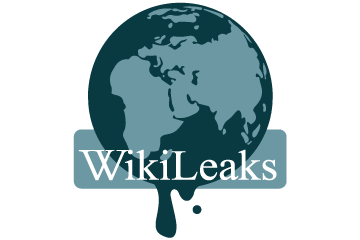
\includegraphics[scale = 0.55]{image2.png}
\end{wrapfigure}

Wikileaks is a media organization founded in 2006 by Julian Assange to
publish original documents from anonymous sources and
leakers.\footnote{Whittaker, Francis. ``What Is WikiLeaks? Everything
  You Need to Know.'' \emph{NBCNews.com}, NBCUniversal News Group, 14
  Aug. 2018,
  www.nbcnews.com/storyline/smart-facts/what-wikileaks-everything-you-need-know-n869556.}
It is regarded as a whistleblowing platform where classified documents
and data sets can be released. A well-known entity in the world of
Internet security, Wikileaks became mainstream in 2010 with the release
of an annotated video called ``Collateral Murder'' that showed the
deliberate bombing of Iraqi civilians by a U.S. helicopter
crew.\footnote{Madrigal, Alexis C. ``The Beginner's Guide to
  WikiLeaks.'' \emph{The Atlantic}, Atlantic Media Company, 14 Dec.
  2010,
  www.theatlantic.com/international/archive/2010/12/the-beginners-guide-to-wikileaks/67705/.}
Wikileaks was also responsible for the leaking of hundreds of thousands
of documents from the Iraq and Afghanistan wars. The release was
orchestrated with several major newspapers and produced a strong global
reaction.  \\

In 2016, Wikileaks made headlines when it released over 30,000 emails
and attachments sent to and from Hillary Clinton's private email server
while she served as Secretary of State under President Barack
Obama.\footnote{``Submit Documents to WikiLeaks.'' \emph{WikiLeaks},
  wikileaks.org/clinton-emails/?q=.} While the fact that Clinton used an
private, nongovernmental email server for official State Department
business was first revealed in 2015, the release of the actual content
of many of the emails by Wikileaks renewed scrutiny on Clinton's risky
handling of classified information.\footnote{Eder, Steve. ``\,'We Need
  to Clean This Up': Clinton Aide's Newly Public Email Shows Concern.''
  \emph{The New York Times}, The New York Times, 25 Oct. 2016,
  www.nytimes.com/2016/10/26/us/politics/wikileaks-hillary-clinton-emails.html.}
This has ultimately played a role in the public perception of Clinton
amid the backdrop of the 2016 Presidential Election. Donald Trump,
Clinton's Republican challenger, has quickly seized on this new
development to criticize his opponent. \\

Wikileaks has proven to be a relevant player in the leadup to the 2016
Presidential Election. Its premise, leaking confidential files to the
public, is of great concern to the FBI. It remains to be seen what the
role of Wikileaks will be moving forward into 2016 in regards to the
election, but it is certainly a group the FBI should monitor. \\

\subsection{2016 Political Climate}

\begin{wrapfigure} {r} {0pt}
\centering
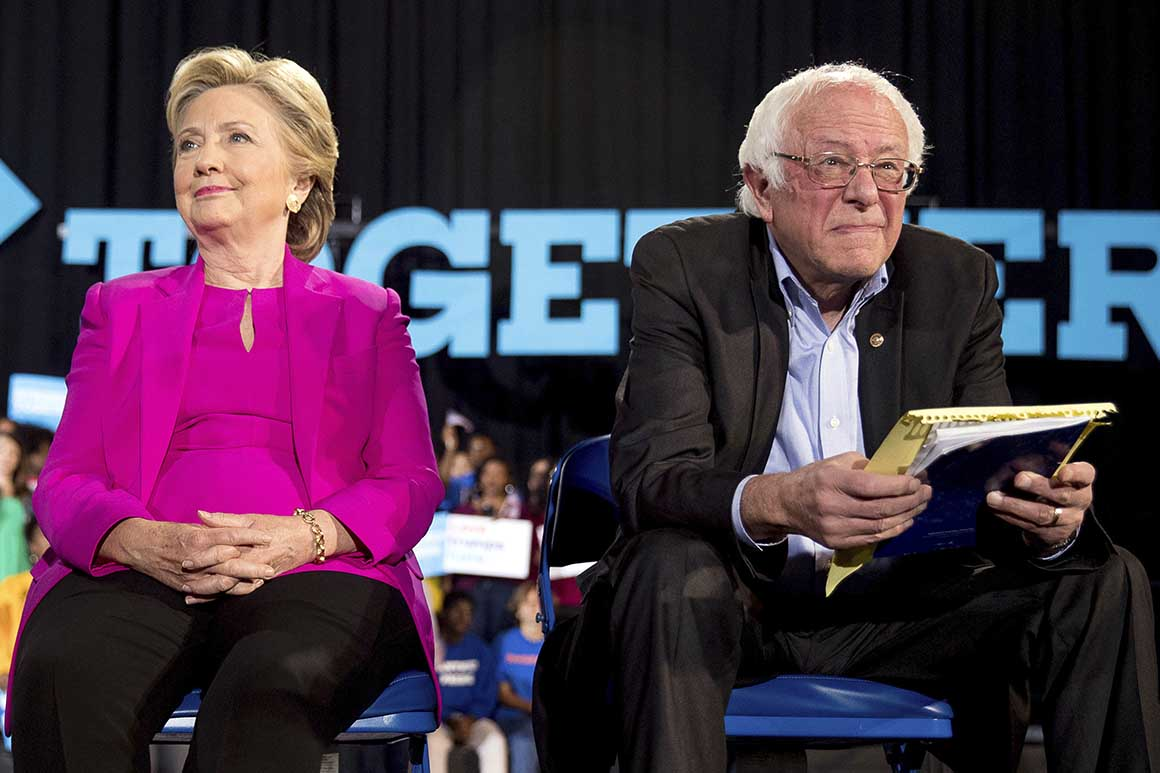
\includegraphics[width=3.42969in,height=2.28646in]{image3.jpg} \\
\end{wrapfigure}
The United States finds itself in a showdown between the presumptive
Democrat nominee Hillary Clinton and the Republican Donald J. Trump, but
that wasn't always the case.

As of the start of this committee, Senator Bernie Sanders of Vermont has
yet to suspend his campaign, although the math suggests he has not
garnered enough votes or delegates to be the Democratic nominee. He
trails Clinton by millions in the Democratic popular vote, and by
hundreds in delegate counts with or without superdelegates. Sanders has
faced public pressure to drop out of the race and endorse Hillary
Clinton in order to unite the Democratic Party against Donald Trump, but
thus far has vowed to continue with his campaign. Either way, Clinton
was recently declared the ``presumptive nominee'' and is now campaigning
as a nominee would, even garnering the support of sitting president
Barack Obama.\footnote{Sanders, Sam. ``Bernie Sanders, Party Crasher:
  Notes On The (Looming) End Of A Campaign.'' \emph{NPR}, NPR, 15 June
  2016,
  www.npr.org/2016/06/15/481453188/bernie-sanders-party-crasher-notes-on-the-looming-end-of-a-campaign.} \\

She campaigns against the presumptive Republican nominee Donald J.
Trump. The Republican field started with 17 candidates, including
household names such as Texas Senator Ted Cruz, Florida Senator Marco
Rubio, and former Florida Governor Jeb Bush.\footnote{History.com
  Editors. ``The 2016 U.S. Presidential Election.'' \emph{History.com},
  A\&E Television Networks, 29 Nov. 2018,
  www.history.com/topics/us-presidents/us-presidential-election-2016.}
Originally considered a political outsider, Trump developed an
enthusiastic voter base with a promise to ``Make America Great Again''
and ran off a string of Republican primary wins. By May 4, Trump became
the presumptive Republican nominee after Kasich suspended his campaign a
day after Trump's victory in the Indiana primary.\footnote{Kaplan,
  Thomas. ``John Kasich Suspends Campaign for President.'' \emph{The New
  York Times}, The New York Times, 4 May 2016,
  www.nytimes.com/2016/05/05/us/politics/john-kasich.html.} \\

Both presumptive nominees have faced their fair share of controversies
on the road to securing their party's respective nomination. As
mentioned before, Clinton has endured heavy criticism for using a
personal email server while serving as Secretary of State. On July 10,
2015, the FBI officially opened a criminal investigation code-named
``Midyear Exam'' on her potential mishandling of classified
information.\footnote{Jarrett, Laura. ``Key Dates in the FBI Probe of
  Hillary Clinton's Emails.'' \emph{CNN}, Cable News Network, 14 June
  2018,
  www.cnn.com/2018/06/14/politics/key-dates-fbi-hillary-clinton-emails/index.html.}
That investigation will still be ongoing at the start of committee.
Clinton has also faced continuous criticism from Republicans over her
handling of the 2012 attack on a U.S. Consulate in Benghazi, Libya that
resulted in the death of four Americans, including Ambassador Chris
Stevens. At the time that committee starts, the House of Representatives
is currently investigating security preparations at the American
facility in Benghazi and how Clinton responded during the night of the
attacks.\footnote{Graham, David A. ``From Whitewater to Benghazi: A
  Clinton-Scandal Primer.'' \emph{The Atlantic}, Atlantic Media Company,
  6 Nov. 2016,
  www.theatlantic.com/politics/archive/2016/11/tracking-the-clinton-controversies-from-whitewater-to-benghazi/396182/.}
Both the FBI and House have yet to release their respective reports on
Clinton's behavior, but the controversy and speculation regarding her
past record has generated questions about her trustworthiness and
presidential merits. \\

 \begin{wrapfigure} {l} {0pt}
 \centering
 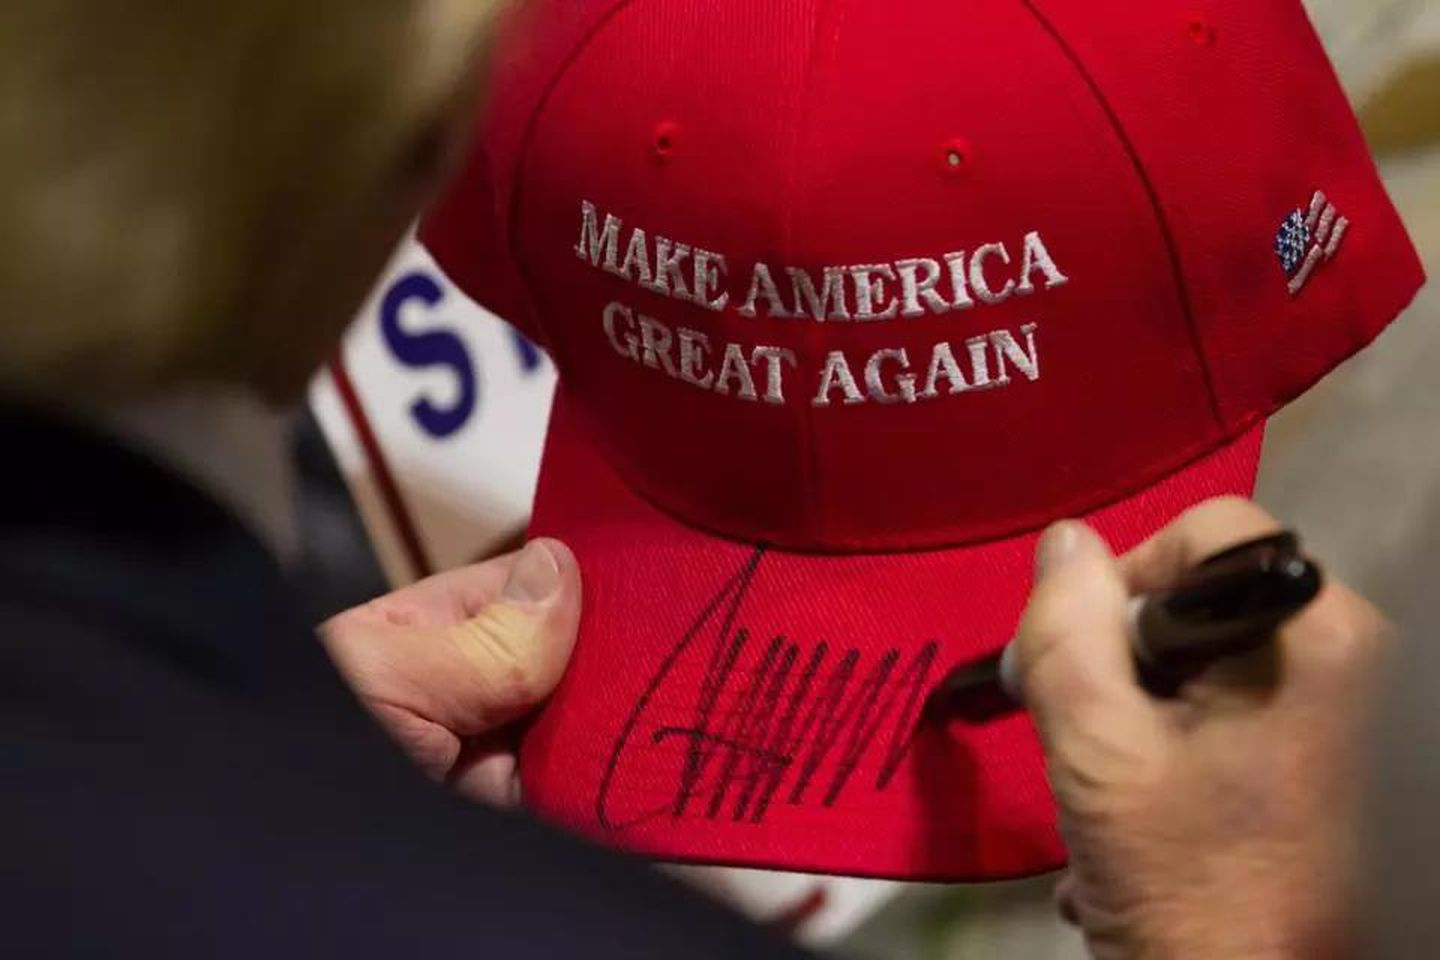
\includegraphics[scale = 0.15]{image5.jpg} 
 \end{wrapfigure}
 
Meanwhile, Trump for years has been a proponent of the ``birther''
theory that current President Barack Obama was not born in the United
States despite it being debunked multiple times.\footnote{Barbaro,
  Michael. ``Donald Trump Clung to 'Birther' Lie for Years, and Still
  Isn't Apologetic.'' \emph{The New York Times}, The New York Times, 16
  Sept. 2016,
  www.nytimes.com/2016/09/17/us/politics/donald-trump-obama-birther.html.}
In addition, even when he announced his campaign on June 16, 2015, he
made headlines for saying Mexican immigrants are ``bringing drugs.
They're bringing crime. They're rapists. And some, I assume, are good
people.''\footnote{Stracqualursi, Veronica. ``7 Of the Most
  Controversial Lines of the 2016 Election.'' \emph{ABC News}, ABC News
  Network, 29 Oct. 2016,
  abcnews.go.com/Politics/controversial-lines-2016-election/story?id=42886273.}
His remarks have been labelled as racist, but his comments on
immigration at our southern border are consistent with his controversial
policy desire of building a wall between the U.S. and Mexico. He has
also faced backlash by calling for an immigration ban that specifically
pertained to Muslims.\footnote{``Donald Trump Urges Ban on Muslims
  Coming to US.'' \emph{BBC News}, BBC, 8 Dec. 2015,
  www.bbc.com/news/world-us-canada-35035190.} Perhaps the most ongoing
issue surrounding Trump has been his refusal to release his tax records.
Going into this election, there is an unprecedented shroud of secrecy
surrounding his finances, with past candidates being much more
transparent with their personal financial dealings. \\

Amid an election between two of the least popular candidates in modern
political history, it is an opportune time for America's foreign
adversaries to attempt to further sow discord. Russia has taken the lead
in this endeavor, with Russian hackers acting to damage the Clinton
campaign, boost Trump's election chances, and most importantly, increase
distrust in the American democratic system.\footnote{Abrams, Abigail.
  ``Here's What We Know So Far About Russia's 2016 Meddling.''
  \emph{Time}, Time, 18 Apr. 2019,
  time.com/5565991/russia-influence-2016-election/.} There have already
been small instances of Russian interference in this election. In
September 2015, an agent from the FBI's Washington Field Office notified
the Democratic National Committee's IT department that at least one
computer had been compromised by Russian hackers.\footnote{Sciutto, Jim.
  ``How One Typo Helped Let Russian Hackers In.'' \emph{CNN}, Cable News
  Network, 28 June 2017,
  www.cnn.com/2017/06/27/politics/russia-dnc-hacking-csr/index.html.} A
low-level DNC technician ended up scanning the system networks but found
nothing and did not follow up with DNC leadership regarding the FBI's
warning. \\
The impacts of Russia's initial attempts at interfering in the election
remain to be seen, but the message is clear. They are taking advantage
of the polarized political climate in the United States. It is up to
this FBI to protect domestic interests and preserve the tenets of
democracy, whatever the costs. \\

\section{Starting Scenario}

\emph{June 14, 2016, Washington D.C., United States:} \\

Thomas J. Quell, a member of the FBI since the 1980's, has become
accustomed to his morning routine at his rather plain D.C. cubicle.
Quell works on the tip line at the Cyber Division, reading mostly
baseless accusations from trolls on the Internet's darker spaces. He
loves his job and has no plans on retiring soon. It comes with a nice
benefits package and he is always home to his wife, Cindy, by 5:30pm.
Today was not going to be one of those days. As he sipped his tea, he
came across an email labeled ``URGENT: RUSSIA HACKS DNC.'' This seemed
strange; most of Quell's emails pertained to more domestic affairs like
leaked social media passwords by an angry teenager in Florida or
fraudulent advertising from a small business owner in California. Either
way, it was his responsibility to investigate all of these claims. He
clicked on the profile and his eyes widened. ``Internet Research
Agency\ldots{} Russia\ldots{} Donald Trump\ldots{} Democratic Party'' he
whispered to himself as he poured over an incredibly lengthy email. He
did not understand what a lot of it meant, but it became plainly
apparent that this information was both as urgent as described and well
above his pay grade. He quickly forwarded it to his boss, flagging it to
make sure it was the first thing they saw, and promptly made a call to
Cindy - he was going to be late to dinner tonight. Not even 30 minutes
later, the entire Bureau is in a frenzy\ldots{} somewhere in Saint
Petersburg, Russia, a man hunched over his laptop and dozens of monitors
running thousands of lines of code whispers: "perfect." \\

Your goal in this committee is to work within your agency, either the
FBI or the IRA, to either prevent a catastrophe surrounding the 2016 US
presidential election or to create one. You must accomplish this while
increasing your own knowledge and influence over the events unfolding
surrounding the election or beyond into 2016. Because who you know is
everything, this may involve working with other committee delegates to
take down those in the opposing bureau, or perhaps working with people
in different agencies in your own country or abroad. You'll also have to
take into account other societal problems of the day, from the political
instability surrounding the election to international issues like
Brexit. Taking all these factors into account, it's up to you to come
out on top. \\

\newpage
\section{Questions to consider while preparing for the
committee}

\begin{itemize}
\item What was my role during this time and in relativity to this group?

\item Are there any other characters in this committee, or in the other
room, to whom my character might be close? How should I go about working
with these individuals?

\item What types of issues will members of this body most likely encounter?

\item What kind of influence do we want to have as a body on the history of
the time? What do we want to change about the way that history played
out?

\item What is my personal goal in this committee? How do I plan to
accomplish it? What kind of decisions will I make along the way to
achieve this goal?
\end{itemize}

These questions are a good place to start when beginning to craft your
plan for this weekend. They will help you to have a good idea about the
goals of your character and the committee. \\

\newpage
\section{Character List}

\subsection{United States, Federal Bureau of Investigation:}

\begin{enumerate}
\item
  \textbf{Michael Johnson, Director of the International Operations
  Division} - Michael Johnson was promoted to the position of Director
  of the International Operations Division only two months ago, but it
  is the perfect position for his experience. After serving in the army
  for five years, Michael returned home to work in the greater defense
  industry. He bounced around to DoD agencies for several years, but
  found his specialty was international relations and negotiation with
  foreign adversaries. He has worked through disagreements with the
  Russians in the past and expects to succeed in these negotiations
  again.
\item
  \textbf{Peter Brown, Director of the Cyber Division} - Peter Brown has
  always had a knack for technology. He was lucky enough to develop his
  programming skills at the height of the tech bubble in the 90s,
  working at IBM and Microsoft before switching gears and working in
  cybersecurity for a major defense contractor. He quickly became
  Northrop Grumman's top code breaker and was snatched up by the FBI.
  For all things code, Peter is the main man for the job.
\item
  \textbf{Thomas Martin, Director of the Criminal Investigative
  Division} - Thomas Martin has worked in the FBI for more than 20 years
  and is next in line to take over as Executive Assistant Director for
  Criminal, Cyber, Response and Services, the overarching branch that
  covers the Cyber Division, International Operations Division, Critical
  Incident Response Group, and the Criminal Investigative Division,
  which he currently leads. With his previous experience as a lawyer, he
  plans to lead his team to investigate any legal repercussions for the
  presidential campaigns or any affiliated individuals.
\item
  \textbf{David Moore, Director of the Critical Incident Response Group}
  - David Moore has been handling crises his whole life. He has been
  working for the FBI since he graduated college, starting as a
  translator for Czech, Russian, and Arabic, becoming a hostage
  negotiator, and then working his way through the ranks to his current
  position. Moore's team was the first to be notified about any direct
  Russian attack on the DNC, and as the problem has snowballed, much of
  the pressure is on him to handle the incident and its effects.
\item
  \textbf{Susan Taylor, Assistant Director of the Cyber Division} -
  Susan Taylor currently serves as the second-in-command of the Cyber
  Division of the FBI, a position that no woman has ever held. She was
  initially hired by the CIA when she hacked into one of their servers
  at age 23, and has taken a few other jobs throughout the intelligence
  community since. Even though she is a talented computer scientist,
  Susan spends most of her time these days leading the Cyber Division to
  accomplish tasks set forth by the director. She is trusted by her team
  because of her no-nonsense leadership style. Her connections across
  D.C. may prove to be her greatest assets in this investigation.
\item
  \textbf{Richard White, Assistant Director of the Criminal
  Investigative Division} - Richard White has been anticipating a
  disinformation campaign or cyber-attack like this one for some time
  now. A former professor of International Law at Columbia Law School,
  White was recruited to the FBI about 5 years ago after they read his
  research. White has been speculating with his fellow professors about
  the weaknesses of the current election system, but he never expected
  to be at the forefront of the problem. Hopefully he can apply his
  research into action. The fate of US elections depends on it.
\item
  \textbf{Lisa Clark, Assistant Director of the Critical Incident
  Response Group} - Lisa Clark has handled crisis after crisis with the
  FBI, but she's never seen anything like this. Lisa is known for always
  being cool in a crisis. Her background in Economics and Management
  allow her to look at the numbers objectively and lead her team
  effectively. Lisa has a husband who works for the CIA, as well as twin
  children, Jeffrey and Jordan, age 5.
\item
  \textbf{Mark Stetson, Assistant Director of the International
  Operations Division} - Mark Stetson is the Assistant Director of the
  International Operations Division of the FBI. Mark is a retired
  operative from the FBI, mostly based in former Societ bloc states. He
  was heavily involved on the ground during the Yugoslavian civil war,
  and his years of covert operations have given him an edge. He is a
  cold and calculating leader who wants nothing more than to get the job
  done and go home to his dog.
\item
  \textbf{Greg Leschnik, Intern in the International Operations
  Division} - A 3rd-year International Affairs and Russian double-major
  at the University of Georgia, Greg scored the internship of a lifetime
  this summer. He just received his security clearance and has been
  assigned introductory work in the International Operations Division.
  In between struggling to learn acronyms for international
  organizations, Greg has decided that if he wants a full-time offer for
  after graduation, he'll need to do everything he can to shine on the
  job. He plans to wow his team with his excellent translation skills
  and knowledge of global issues that he gained as a member of the UGA
  Model UN team.
\item
  \textbf{David Green, Programmer in the Cyber Division} - David Green
  is perhaps the strongest programmer in the Cyber Division, but he
  doesn't have much to show for it. At 32, he hasn't yet gotten married
  (or even even had a significant other), but his rich parents have
  helped him get into the best schools and have the best exposure to
  tech from a young age. His family is also well-connected around town:
  his Dad is a senator from North Dakota. David was groomed for a life
  of politics, but is just too geeky to make it work. His team trusts
  his code, but they never invite him out to drinks after work.
\item
  \textbf{William Byrd, Analyst in the International Operations
  Division} - William Byrd is the most recent hire in the International
  Operations Division. And by recent, we mean \emph{very} recent: this
  is his sixth day on the job. Even after only one week, William is very
  much struggling with this job and thinking about quitting. But just as
  he got up the nerve to talk to his supervisor, he was assigned a major
  part of the investigation into Russian operatives. It's his first
  major task, and he can't really leave now. William isn't quite
  committed to this work, so he has a lot of choices on his hands. Will
  he sell information? Will he backstab his coworkers? Will he do the
  best dang analyst job the world has ever seen? It's up to him.
\item
  \textbf{Brian Davis, Analyst in the Critical Incident Response Group}
  - Brian Davis is an Analyst by trade, but a linguist my passion. He
  studied linguistics in undergrad with a concentration in rhetoric, and
  he has his PhD in Political Psychology from Princeton. Brian loves to
  read through messages and analyze wording for specific clues, phrases,
  and secret messages. His latest job has been working with the cyber
  team to screen social media posts for dangerous trends. Hopefully his
  work with words will be used for good and not for evil.
\item
  \textbf{JP McCall, Analyst in the Cyber Division} - JP McCall has been
  an analyst in the Cyber Division for over 7 years, after working at
  NASA on the security team. Over the same time, he consulted for the
  CIA and the NSA for the Stuxnet virus After working for intelligence
  agencies, he was interested in the more political application of
  intelligence work and decided to move to the State Department for a
  bit. A jack of all trade, JP works well with the team and is happy
  with his work.
\item
  \textbf{Scott Pavinsky, Special Agent in the Criminal Investigative
  Division} - Scott Pavinsky is a small-town boy from Nebraska. Inspired
  by his father, the Chief of Police in Lakeside, he worked as a police
  officer before being hired by the Nebraska Bureau of Intelligence. His
  work was so incredible that he was recruited to the FBI only a few
  years later. Eager to prove his worth in the big city, Scott is
  nervous but excited to get his first major case investigating Russians
  involved in election interference.
\item
  \textbf{Donna Hendrix, Translator in the Critical Incident Response
  Group} - Donna Hendrix is one of the only FBI agents in her division
  that is not from the US. She grew up in Ukraine, so she has lots of
  political thoughts about Russia and their interference in Eastern
  European affairs, but she fell in love with an American named Ryan in
  her teens and moved to DC for him. Donna is an expert translator and
  hopes to climb the ranks to an analyst position over time, but she's a
  bit flighty and reactionary. Her team doesn't really know how to work
  with her, but they know she always does her work ahead of schedule and
  gets the job done well.
\end{enumerate}

\newpage
\subsection{Russia, Internet Research Agency:}

\begin{enumerate}
\item
  \textbf{Boris Alekseyevich Antonov, Major, Unit 26165 -} Boris
  Alekseyevich Antonov has worked hard to get from his small hometown in
  Russia to become a Major in Unit 26165 and a force within GRU. Known
  as a cut-throat military intelligence officer, Boris has worked
  extremely hard to get where he is today. Though not well connected to
  the Kremlin, he has proven his worth through his inventive and unique
  coding abilities. These abilities combined with his charisma make him
  both a friend to all and a serious threat to adversaries.
\item
  \textbf{Dmitriy Sergeyevich Badin, Military Intelligence Officer, Unit
  26165 -} Dmitriy Sergeyevich Badin has always had an affinity for art.
  As a young child, he loved creating different art pieces from
  wonderful pieces of digital art to delicate pottery pieces. These
  creative talents have led Dmitriy to a successful career in Unit
  26165. Though only a military intelligence officer and no true rank,
  Dmitriy has been instrumental in past missions and craves to earn a
  higher rank.
\item
  \textbf{Anatoliy Sergeyevich Kovalev, Military Intelligence Officer,
  Unit 74455 -} Anatoliy Seregyevich Kovalev is newly married and
  enjoying his new assignment in Unit 74455. His wife, Helga, is also in
  Russian military intelligence and often collects information about FBI
  agents. While only an officer, Antoliy has big plans to move up the
  chain of command and eventually lead his unit. However, his wife's
  work and his own possible connections to the FBI may hold him back.
\item
  \textbf{Nikolay Yuryevich Kozachek - Lieutenant Captain, Unit 26165 -}
  Known to some as ``blablabla1234565'' and as Nikolay to others,
  Nikolay Yuryevich Kozachel is the ``class clown'' amongst his
  unit\footnote{\href{https://www.fbi.gov/wanted/cyber/nikolay-yuryevich-kozachek}{\underline{https://www.fbi.gov/wanted/cyber/nikolay-yuryevich-kozachek}}}.
  His pranks are legendary and so are his coding skills. He has been
  able to move up so quickly through the ranks due to ingenuity and
  charisma. However, his pranks sometimes get out-of-hand and cause
  issues with his superior officers. Even still, Nikolay is a hard
  working lieutenant captain with a love of complex problems and
  creating funny solutions.
\item
  \textbf{Aleksey Viktorovich Lukashev, Senior Lieutenant, Unit 26165 -}
  All the way from Murmanskaya Oblast, Russia to the Internet Research
  Agency, Aleksey is known for his exceedingly sharp intellect as well
  as his love for music. As a child, he learned the piano, the violin,
  and, of course, the accordion. He has a knack for coming up with
  catchy, repetitive songs that can get stuck in anyone's head. His life
  dream is to eventually get involved with politics and become President
  of Russia.
\item
  \textbf{Artem Andreyevich Malyshev, Senior Lieutenant, Unit 26165 -}
  Born on February 2, 1988, Artem always knew two things: that he loved
  his home country of Russia and that he was destined for greatness. He
  worked his way up the intelligence ladder to become Senior Lieutenant
  of Unit 26165 (obviously the best unit). Artem's confidence definitely
  helped him reach his current rank, and he's now eager to prove himself
  and his unit to the higher ups.
\item
  \textbf{Sergey Aleksandrovich Morgachev, Lieutenant Colonel, Unit
  261265 -}Sergey started out a mere janitor in the Internet Research
  Agency, but he had big dreams (plus his mother always said he was
  special). After taking a number of coding courses, and using some old
  books to self-learn, he finally managed to reach the rank of
  Lieutenant Colonel of Unit 26165. Despite others fearing the abilities
  of a Ukranian ``janitor,'' Sergey knows he has more to offer and looks
  forward to showing up all these stuck up Russians by being the best at
  his work, and, just maybe, being a leader of the IRA.
\item
  \textbf{Aleksandr Vladimirovich Osadchuk, Colonel, Unit 74455 -}
  Aleksandr always knew he would be a military man, being the son of an
  army officer, but his heart yearned for the written word. Despite his
  desires to follow in his heroes' footsteps, his family pushed him
  towards mathematics and military strategy. Ultimately, he landed in
  the Internet Research Agency as a Colonel and commanding officer of
  Unit 74455. Aleksandr does good work, always a capable and dutiful
  man, but ever does he long to write more than just code.
\item
  \textbf{Aleksey Aleksandrovich Potemkin, Supervisor, Unit 74455 -}
  Aleksey was always a gifted young man; born in March 20, 1983, and
  excelling in mathematics, physics, and computer science, he was
  expected to go straight into academia. However, Aleksey simply did not
  have the money for higher education, but in came the Russian military
  offering a lucrative (and obviously patriotic) position with the IRA.
  Aleksey quickly accepted and now is a military intelligence officer
  and supervisor of Unit 74455. He hopes to prove himself and make
  enough to further his education goals, and that he could get a better
  job elsewhere by doing well in the IRA.
\item
  \textbf{Ivan Sergeyevich Yermakov. Military Intelligence Officer, Unit
  26165 -} Ivan Yermakov, or better known to some as ``Kate S. Milton'',
  ``James McMorgans'', or ``Karen W. Millen'', was born in 1986 and was
  an adept hacker and coder. He always loved messing with people and
  trolling others, especially online, and one day he just happened to
  cross the wrong oligarch. Thankfully though, the man offered Ivan a
  job with the Internet Research Agency doing everything he loved:
  trolling. Ivan became a military intelligence officer in Unit 26165,
  and is content with his job, but he knows he could be doing so much
  more damage if only he was given the chance.
\item 
  \textbf{Pavel Vyacheslavovich Yershov, Military Intelligence Officer,
  Unit 26165, -} Pavel was always a bit on the quieter side, but he was
  smart and hard working. While studying Computer Science in a major
  university in Moscow, Pavel managed to land a job with the Russian
  government. Despite his quiet nature, Pavel managed to get a mentor in
  the intelligence office who helped him get into the Internet Research
  Agency in unit 26165. Pavel hopes to prove his mentor right and break
  out of his shell and finally move beyond the grunt work of the
  intelligence field.
\end{enumerate}

\end{document}
